% Paper 2 -- the SKQD localisation boundary. Every number carries its RESULTS.md row id
% in a LaTeX comment; do not edit numbers here without the ledger. Build:
%   pdflatex main.tex && pdflatex main.tex
% STATUS: full draft, but see Sec. "Work required before submission" -- this paper
% needs additional experiments to survive review; the gaps are listed there explicitly.
\documentclass[a4paper,11pt]{quantumarticle}
\pdfoutput=1
\usepackage[utf8]{inputenc}
\usepackage[T1]{fontenc}
\usepackage{amsmath,amssymb}
\usepackage{graphicx}
\usepackage{booktabs}
\usepackage{hyperref}

\begin{document}

\title{Where sample-based Krylov diagonalisation works: a localisation boundary on exactly solvable models}

% TODO(team): author order, affiliations, and emails are placeholders -- decide before
% submission. All five hackathon members listed alphabetically for now.
\author{Chao Hsien}
\author{Jiwan Kang}
\author{Ng Siu Hin}
\author{Su Wei-Chang}
\author{Tina Tien}
\affiliation{Qiskit Hackathon 2026, Team 8 --- affiliation TBD}

\maketitle

\begin{abstract}
Sample-based quantum diagonalisation methods (SQD, and its Krylov variant SKQD) project
a Hamiltonian into the span of computational-basis configurations sampled from
quantum-prepared states, betting that a modest number of sampled configurations captures
the ground state. We map where that bet pays on exactly solvable spin and fermion
models, where every quantity can be graded against exact diagonalisation. The governing
parameter is ground-state localisation. On half-filled charge sectors of an XXZ chain
(sector dimension up to 3\,432) the sampled-subspace fraction required for
$1\%$ ground-energy accuracy \emph{falls} from $84\%$ to $2.7\%$ of the sector as the
Ising anisotropy $\Delta/J$ grows from $0.38$ to $5$ --- a monotone boundary confirmed
across 20 sampling seeds with bootstrap confidence intervals.
% R047, R057
The same boundary reappears on a $2\times3$ Fermi--Hubbard lattice as a function of
$U/t$: convergence is never reached in the metallic regime ($U/t\leq4$), while the Mott
regime needs only $12.5\%$ of the sector at $U/t=16$.
% R050
Geometry acts through the same axis: added connectivity worsens sampling only where
hopping already dominates, and is irrelevant once the ground state is localised.
% R048
Separately, we observe that the method's premise (a concentrated ground state) and its
success (sampling \emph{finding} that concentration) can fail independently: on the
delocalised side, the fraction of the sector needed \emph{rises} with system size even
as the ground state's weight concentrates. These boundaries are consistent with why
sample-based methods succeed in quantum chemistry, where a dominant reference
configuration places the problem on the localised side of the axis.
\end{abstract}

\section{Introduction}
\label{sec:intro}

Sample-based quantum diagonalisation (SQD)~\cite{sqd} and its Krylov-inspired variants
(SKQD)~\cite{skqd} occupy a pragmatic middle ground in near-term quantum simulation:
the quantum processor is used only to \emph{sample computational-basis configurations}
from prepared states, and a classical solver diagonalises the Hamiltonian projected
onto the span of the sampled configurations. The approach tolerates hardware noise
gracefully --- a corrupted sample is just a possibly-irrelevant basis state --- and has
produced striking demonstrations in quantum chemistry.

Its central bet, however, is rarely tested where it can be graded exactly: that a
tractable number of sampled configurations spans the ground state. This paper maps
where that bet pays, on models small enough that every claim is checked against exact
diagonalisation, yet structured enough (conserved charge, tunable
localisation, tunable geometry, and a fermionic analogue) that the answer has a
mechanism rather than an anecdote.

Our results are simply stated. The governing parameter is \emph{ground-state
localisation} in the computational basis. Tune it --- by Ising anisotropy $\Delta/J$ on
a spin chain, or by interaction strength $U/t$ on a Fermi--Hubbard lattice --- and the
sampled-subspace fraction required for fixed accuracy sweeps from ``essentially the
whole sector'' to ``a few percent''. Geometry (1D versus 2D at identical Hilbert-space
dimension) matters only on the delocalised side. And on that delocalised side the
required \emph{fraction} of the sector grows with system size even though the ground
state's weight concentrates --- the premise of the method and its success are separable,
and the gap between them is exactly the ranking quality of the sampler.

We state the scope plainly: sectors up to dimension 3\,432, one spin family and one
fermion family, sampling simulated from exact statevectors (supplemented by one
real-hardware configuration-recovery experiment), and single-seed measurements
everywhere except the central $\Delta/J$ sweep, which carries 20 seeds and bootstrap
confidence intervals. Section~\ref{sec:todo} lists the additional experiments we
consider necessary before these boundaries should be treated as more than a
well-controlled small-scale map.

\section{Protocol}
\label{sec:protocol}

The spin family is an open XXZ chain,
$H=\sum_i [J(X_iX_{i+1}+Y_iY_{i+1})+\Delta Z_iZ_{i+1}]+\sum_i h_iZ_i$, $J=0.65$, fixed
local fields, with conserved charge $Q=\sum_iZ_i$; all experiments run inside the
half-filled sector, of dimension $\binom{n}{n/2}$: 252 ($n=10$), 924 ($n=12$), 3\,432
($n=14$). The sector Hamiltonian is validated against the full $2^n$ matrix before
anything is measured (elementwise agreement $0.0$; ground energies identical to 8
decimals at $n=4,6$).
% R047

The protocol is SQD's actual one rather than a strawman: prepare a reference
configuration (the N\'eel state, or the lowest-diagonal configuration of $H$ --- the
spin-model analogue of a Hartree--Fock reference), evolve it to a grid of times, sample
configurations from the time-evolved states (3\,000 draws per time, ten times), rank
configurations by observed frequency, and diagonalise $H$ restricted to the span of the
top-$M$. The reported quantity is the smallest $M$ (as a fraction of the sector) whose
ground energy is within $1\%$ of the exact sector ground energy --- relative to $|E_0|$
for the spin models, and relative to the sector \emph{bandwidth} for Hubbard, where
$E_0\to0$ at large $U/t$ makes a relative-to-$|E_0|$ threshold measure the metric
rather than the method (a bug we hit and record).
% R047, R050

The fermionic family is a $2\times3$ Fermi--Hubbard lattice at half filling
($N_\uparrow=N_\downarrow=3$, 12 qubits, sector dimension 400), mapped by an explicitly
validated Jordan--Wigner construction: $[H,N_\uparrow]=[H,N_\downarrow]=0$ exactly; at
$U=0$ the full many-body spectrum matches the free-fermion prediction to
$1.9\times10^{-15}$; at $t=0$ every eigenvalue is an exact integer multiple of $U$.
% R050

\section{The localisation boundary}
\label{sec:boundary}

\begin{figure*}[t]
  \centering
  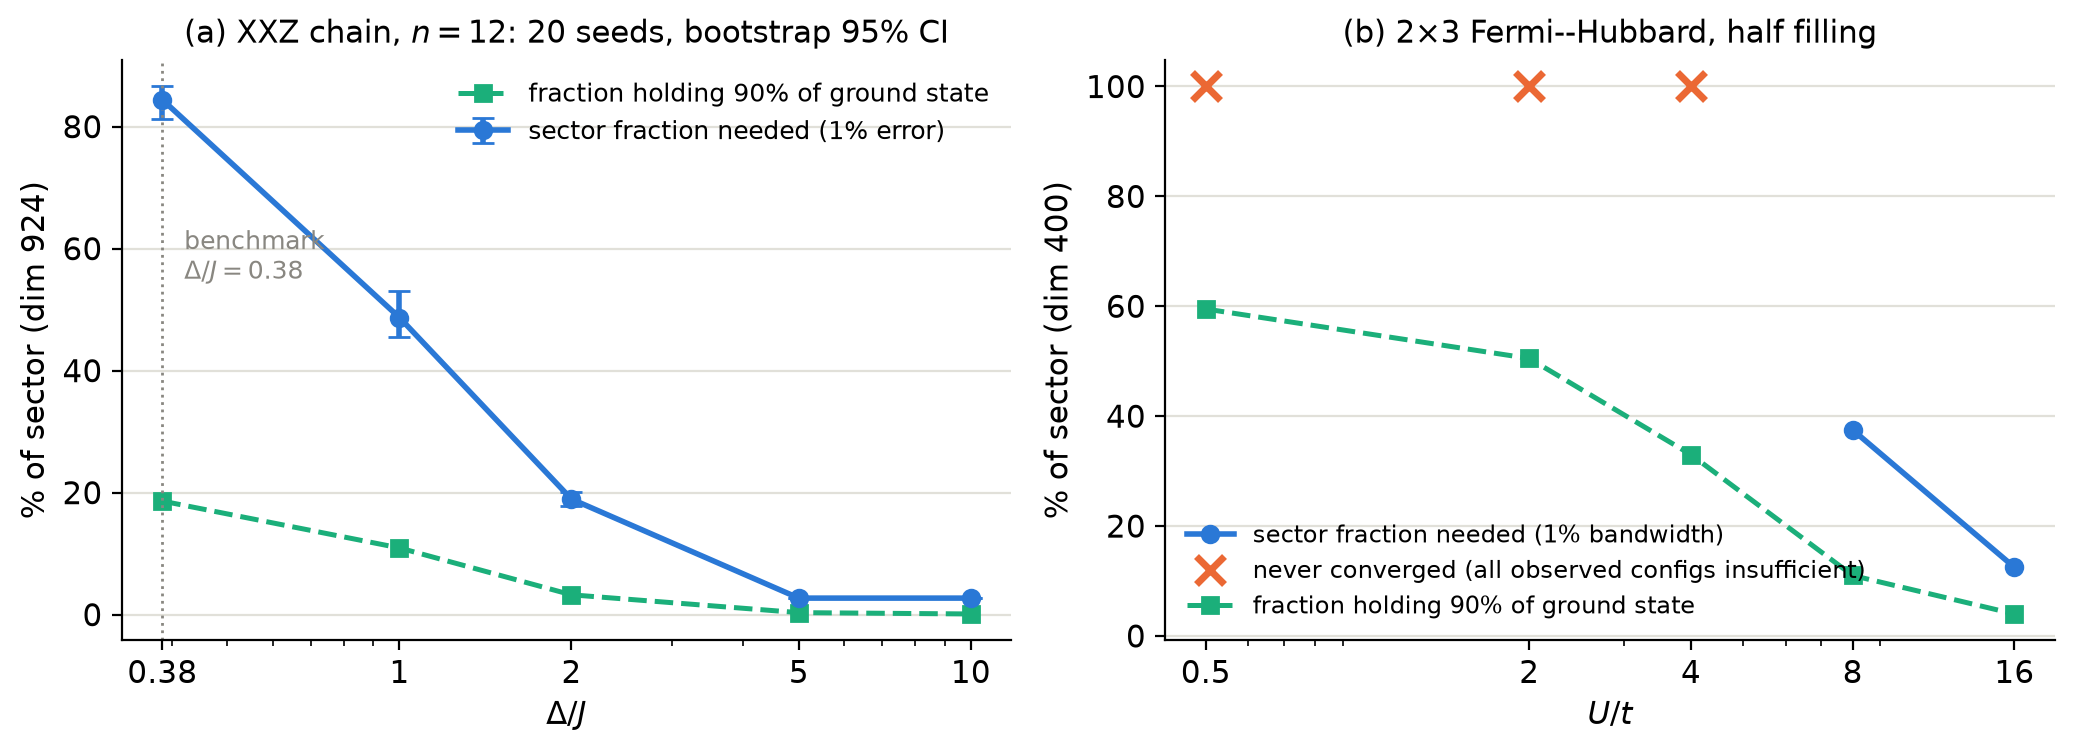
\includegraphics[width=0.95\textwidth]{fig_boundary_ci_hubbard.png}
  \caption{The localisation boundary. (a)~XXZ chain, $n=12$ half-filled sector
  (dimension 924): sector fraction needed for $1\%$ ground-energy error versus
  $\Delta/J$, mean over 20 independent sampling seeds with bootstrap $95\%$ confidence
  intervals, alongside the fraction of the sector holding $90\%$ of the exact ground
  state. (b)~The same boundary on the $2\times3$ Fermi--Hubbard lattice at half filling
  (sector dimension 400) as a function of $U/t$; crosses mark points where no sampled
  subspace --- including the span of \emph{every} configuration the sampler observed ---
  reached the target.}
  \label{fig:boundary}
\end{figure*}

\emph{Spin chain.} At the hopping-dominated point $\Delta/J=0.38$ the $n=12$ sector
requires $84.4\%$ $[81.2,86.6]\%$ of its 924 configurations for $1\%$ accuracy; at
$\Delta/J=1$, $48.7\%$ $[45.5,53.0]\%$; at $\Delta/J=2$, $18.9\%$ $[17.9,20.0]\%$; and
by $\Delta/J\geq5$ the requirement collapses to $2.7\%$ with zero variance across all
20 seeds (every seed converges at the smallest subspace probed). The decrease is
monotone across the sweep (verified programmatically, not by eye).
% R057
Fig.~\ref{fig:boundary}(a) shows both this requirement and the underlying ground-state
concentration.

\emph{Fermi--Hubbard.} The same axis, relabelled $U/t$
[Fig.~\ref{fig:boundary}(b)]: in the metallic regime ($U/t=0.5$, $2$, $4$) the target
is \emph{never} reached --- not even in the span of every configuration the sampler
observed (278, 398, 395 of 400 respectively) --- while the Mott regime needs $37.5\%$
at $U/t=8$ and $12.5\%$ at $U/t=16$, where $90\%$ of the ground state lives on $11\%$
and $4\%$ of the sector.
% R050
This is, we believe, the practically relevant statement of why sample-based
diagonalisation succeeds in chemistry~\cite{sqd}: those systems sit at the localised
end of exactly this axis, with a Hartree--Fock determinant dominating the ground state.

\emph{Geometry is the same knob, not a new one.} Comparing a 12-site chain (11 bonds)
against a $3\times4$ grid (17 bonds) at identical sector dimension 924: in the
delocalised regime added connectivity strictly hurts (at $\Delta/J=0.38$ the 2D ground
state spreads over $44\%$ of the sector against 1D's $19\%$, and 2D never reaches the
target at all), while in the localised regime ($\Delta/J\geq2$) the two geometries are
\emph{identical} (16.2\% and 2.7\% in both) --- once the ground state collapses onto a
handful of configurations, how they are connected no longer matters.
% R048

\section{Premise and success are separable}
\label{sec:separable}

A subtlety worth its own section: on the delocalised side, the method's premise
\emph{improves} with system size while its performance \emph{degrades}. Across
$n=10,12,14$ at $\Delta/J=0.38$, the fraction of the sector holding $90\%$ of the
ground state falls ($24.2\%\to18.6\%\to14.1\%$ --- concentration, exactly what the
method assumes), yet the fraction required for $1\%$ accuracy rises
($79.4\%\to86.6\%\to93.2\%$).
% R047
The gap between those two curves is the ranking quality of the sampler: time-evolved
reference states visit the important configurations, but do not visit them
\emph{preferentially enough} for a frequency ranking to put them first. Any proposal to
push sample-based methods into delocalised regimes must attack the ranking, not the
concentration.

Two methodological cautions from our own false starts, recorded because both faked a
different conclusion before being caught. First, pooling every configuration a fixed
shot budget happens to observe (rather than ranking by frequency and truncating)
measures the sampler's coverage, not the method, and made the failure look far worse
than it is. Second, on Hubbard, an accuracy threshold relative to $|E_0|$ tightens
without bound at large $U/t$ (where $E_0\sim -t^2/U\to0$) and reported ``never
converged'' even in the trivially-localised regime; rescaling to the sector bandwidth
restored a metric comparable across the axis.
% R047, R050

\section{Contact with hardware}
\label{sec:hardware}

The boundary above is measured with sampling simulated from exact statevectors, which
isolates the method from device noise. One ingredient has been exercised on real
hardware: configuration recovery. Using 36\,000 shots of a genuine random-basis shadow
ensemble on \texttt{ibm\_kingston} (a 2-site reduced instance), $1.65\%$ of all-$Z$
shots violated charge conservation and were identified \emph{without any reference
state or simulation}; symmetry-based configuration recovery then removed exactly that
corruption from a downstream spectral estimate.
% R023, R036, R037
This supports the standard claim that sample-based pipelines degrade gracefully under
hardware noise, but we emphasise it does not test the localisation boundary itself on
hardware.

\section{Work required before submission}
\label{sec:todo}

% TODO(team): this section is the honest work-list; it should shrink to nothing and be
% deleted as the items are done. Referees will ask for all of it.
We record, deliberately in the manuscript itself at this stage, what this study still
needs before the boundary map should be treated as established beyond well-controlled
small instances:
\begin{enumerate}
  \item \textbf{Seeds everywhere.} Only the central $\Delta/J$ sweep carries 20 seeds
  and bootstrap intervals; the size scan, geometry comparison, and Hubbard sweep are
  single-seed and need the same treatment.
  % R047, R048, R050 vs R057
  \item \textbf{Larger sectors.} Dimension $3\,432$ is far from the regime where
  sample-based methods claim value; the trend in Sec.~\ref{sec:separable} should be
  followed at least another order of magnitude (sparse sector construction makes
  $n=16$--$20$ feasible classically).
  \item \textbf{Reference-state study.} The N\'eel-versus-lowest-diagonal comparison
  was inconclusive at our sizes (the references coincide at $n=10,12$); a genuine
  Hartree--Fock-like family of references with tunable ground-state overlap would turn
  the chemistry analogy from plausible to demonstrated.
  \item \textbf{Comparison against production SQD implementations,} including their
  configuration-recovery and self-consistent iteration machinery, on the same models
  --- our top-$M$-by-frequency protocol is deliberately minimal.
  \item \textbf{Direct engagement with the chemistry literature:} at least one small
  molecular system placed on the same localisation axis, so the boundary connects to
  the regime where these methods are actually used.
\end{enumerate}

\section{Discussion}
\label{sec:discussion}

The practical output of this study is a placement rule: before applying a sample-based
diagonalisation method, estimate where the problem sits on the localisation axis ---
$\Delta/J$-like anisotropy for spins, $U/t$ for fermions, reference-configuration
dominance in general. On the localised side the methods are excellent and geometry is
irrelevant; on the delocalised side the required subspace approaches the full sector,
worsens with connectivity and with size, and the bottleneck is the sampler's ranking
rather than the ground state's concentration. None of this contradicts the reported
chemistry successes --- it locates them.

All claims here are graded against exact diagonalisation on purpose, and no advantage
over classical computation is claimed anywhere.

\section*{Data and code availability}
All scripts, evidence files, and the results ledger sourcing every number here (row
identifiers embedded as comments in the manuscript source) are public at
\url{https://github.com/mnsh0409/Qiskit-Hackathon-2026}.

\section*{Acknowledgments}
% TODO(team): funding, IBM Quantum access acknowledgment wording, hackathon organisers.
This work was carried out as part of the Qiskit Hackathon 2026 (Topic~5). We acknowledge
the use of IBM Quantum services; the views expressed are those of the authors and do not
reflect the official policy of IBM or the IBM Quantum team.

\begin{thebibliography}{9}
% All entries verified 2026-08-16 against the arXiv abstract pages / journal records.
\bibitem{sqd} J. Robledo Moreno \emph{et al.},
\emph{Chemistry beyond the scale of exact diagonalization on a quantum-centric
supercomputer}, Sci. Adv. \textbf{11}, eadu9991 (2025); arXiv:2405.05068.

\bibitem{skqd} J. Yu, J. Robledo Moreno, J.~T. Iosue \emph{et al.},
\emph{Quantum-centric algorithm for sample-based Krylov diagonalization},
arXiv:2501.09702 (2025).

\bibitem{faehrmann2025} P.~K. Faehrmann, J. Eisert, and R. Kueng,
\emph{In the shadow of the Hadamard test: Using the garbage state for good and further
modifications}, Phys. Rev. Lett. \textbf{135}, 150603 (2025); arXiv:2505.15913.

\bibitem{huang2020} H.-Y. Huang, R. Kueng, and J. Preskill,
\emph{Predicting many properties of a quantum system from very few measurements},
Nat. Phys. \textbf{16}, 1050 (2020).

\bibitem{qiskit} A. Javadi-Abhari \emph{et al.},
\emph{Quantum computing with Qiskit}, arXiv:2405.08810 (2024).
\end{thebibliography}

\end{document}
